\section{Problemstellung}
Als Spielleiter verliere ich viel Zeit mit dem zusammensuchen von Textpassagen in den entsprechenden Regelbüchern.\\
Themenbereiche sind meist über mehere Bücher verteilt und bieten Alternativregeln welche nicht immer im jeweiligen Inhaltsverzeichnis als solche gekennzeichnet oder überhaupt referenziert sind.\\

\begin{figure}
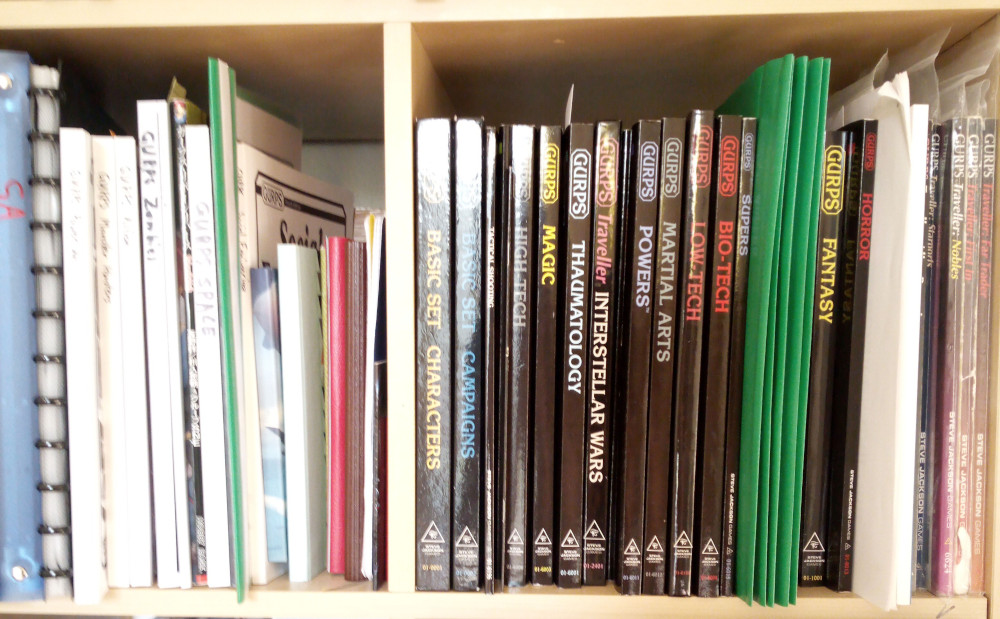
\includegraphics[width=\textwidth]{regal.jpg}
\caption{Büchersammlung}
\end{figure}

\section{Lösungskonzept}
\subsection{Grobbeschreibung}
Ziel ist die Entwicklung einer Referenzdatenbank in welcher Regelbereiche und ihre dazugehörigen Buchreferenzen verwaltet (erfasst, geändert und gelöscht) werden können.\\
Die Applikation sollte in einer Auflistung der Regelbereiche starten welche gefiltert werden können. Per Auswahl des Regelbereichs sollen die jeweiligen Referenzen ersichtlich werden.\\ Bücher und Referenzen sollten getrennt erfasst werden können um die Daten zu normalisieren.
\newpage
\subsection{Use case}
\begin{figure}

\includegraphics[width=\textwidth]{usecase.png}
\caption{Use case zeigt die drei Verwaltungs-Cases}
\end{figure}
Jeder der drei Verwaltungs-Cases ermöglicht es die jeweilige Ressource zu erstellen, bearbeiten und zu löschen.\\
Für jeden Case werden je eine Übersichtsliste und eine Detailansicht benötigt.\\
\paragraph{Regelbereich verwalten}
Der Benutzer kann in der Hauptliste neue Regelbereiche durch einen Menüpunkt anlegen.\\
Der Benutzer kann in der Regelbereich-Detailansicht den entsprechenden Regelbereich löschen, dabei bleiben Referenzen unberührt.\\
Der Benutzer kann in der Regelbereich-Detailansicht die Informationen des Regelbereichs (Bezeichnung, Beschreibung, ...) anpassen.
\paragraph{Referenz verwalten}
Der Benutzer kann eine neue Referenz in der Regelbereich-Detailansicht oder in der Buch-Detailansicht anlegen.\\
Der Benutzer kann über die Referenz-Detailansicht die entsprechende Referenz löschen.\\
Der Benutzer kann über die Referenz-Detailansicht die Informationen der Referenz (Seitennummer, Notizen, ...) anpassen.
\paragraph{Buch verwalten}
Der Benutzer kann über die Buch-Übersichtsliste ein neues Buch anlegen.\\
Der Benutzer kann über die Buch-Detailansicht das entsprechende Buch nur löschen, wenn alle dazugehörigen Referenzen gelöscht wurden.\\
Der Benutzer kann über die Buch-Detailansicht die Informationen des Buches (Name, Author, Erscheinungsjahr, ISBN, ...) anpassen.
\newpage
\subsection{Klassendiagram}
\begin{figure}

\includegraphics[width=\textwidth]{simpleclasses.png}
\caption{Grobes Klassendiagram zeigt die drei Hauptkomponenten (Regelbereich, Referenz und Buch) und ihre Verknüpfung}
\end{figure}
Drei Entity-Klassen wurden identifiziert: Regelbereich, Referenz und Buch.\\
Referenzen gehören immer zu einem bestimmten Buch.\\
Eine Referenz kann in mehreren Regelbereichen referenziert werden.